

%_____
\pagebreak
\section*{Fitting models for nonlinear trends}

Prerequisites: Sections~1.1-1.6, 3.1, 4.1-4.4, 7.1-7.4, and~8.1 from \href{http://www.openintro.org/stat/textbook.php}{OpenIntro Statistics} are the bare minimum.

Figure~\ref{nonlinear} presents two examples of nonlinear relationships between two numerical variables. We'll introduce two techniques for fitting these two data sets: (1)~transforming the response variable and (2)~fitting nonlinear model using polynomial terms in multiple regression. While these two methods are very useful, there is no ``one size fits all'' modeling solution, and there are plenty of situations where these two methods will be insufficient for your needs. If you find that nonlinearity or challenges with residuals cannot be adequately addressed using these methods, consider turning to additional statistical methods.\footnote{See the \href{http://www.openintro.org/stat/supplements.php?feature=regression_online_extra_more_free_books}{Supplement page on openintro.org} for recommended free books that may be useful, or post a question on the online \href{http://www.openintro.org/stat/forums.php}{Public Forums on openintro.org}.}

\begin{figure}[h]
\centering
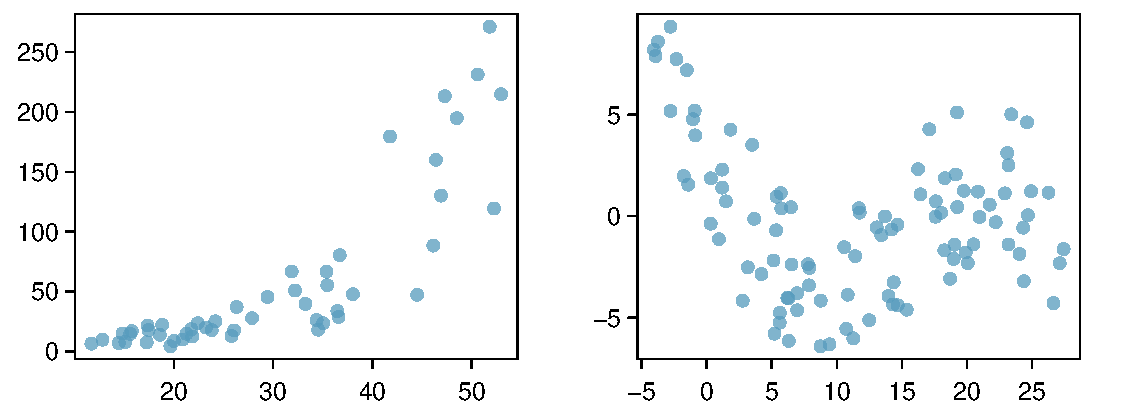
\includegraphics[width=\textwidth]{RegressionExtras/figures/nonlinear/nonlinear} 
\caption{Two pairs of numerical variables where each relationship is nonlinear. The residuals may also show other deviations that must be considered when modeling these data, including non-normal or \term{heteroskedastic} residuals (\emph{heteroskedastic} means \emph{non-constant variance}).}
\label{nonlinear}
\end{figure}

The techniques introduced in this section may be useful when the first, second, or fourth conditions for a simpler linear model are violated:
\begin{enumerate}
\setlength{\itemsep}{0mm}
\item the model residuals should be nearly normal,
\item the variability of the residuals is nearly constant,
\item the residuals are independent, and
\item each variable is linearly related to the outcome.
\end{enumerate}

\subsection{Transformations on the response}

Consider the scatterplot in the left panel of Figure~\ref{nonlinear}. Here, the response $y$ (vertical) tends to be positive but grow quickly. Additionally, the residuals show non-constant variance, because they are more variable for larger values of $x$ (horizontal) and $y$. These two characteristics of the untransformed data are a clue that a~transformation may be~useful.

In Section~1.6 of \href{http://www.openintro.org/stat/textbook.php}{OpenIntro Statistics}, we learned about the power of transformations to make skewed data more symmetric. If we look at a histogram of the $x$ and $y$ variables in Figure~\ref{nonlinear1-2}, we can see that $x$ shows a very slight right skew and $y$ is strongly right skewed. This suggests that it may be useful to transform the $y$ variable. Had $x$ been strongly right skewed, then we should have also considered using a transformation on $x$.

There are many possible transformations, but one of the most common is the natural log-transformation (sometimes written as $ln$). We'll take the natural log for the $y$ values and call this new variable~$y^\star$:
\begin{align*}
y^\star = \log y\text{, where ``log'' is the natural log}
\end{align*}
Figure~\ref{nonlinear1-3} shows $y^\star$ plotted against $x$. The data now show a linear relationship, where outliers are limited and the variability is roughly constant. Such an outcome is ideal, though far from guaranteed.

\begin{figure}
\centering
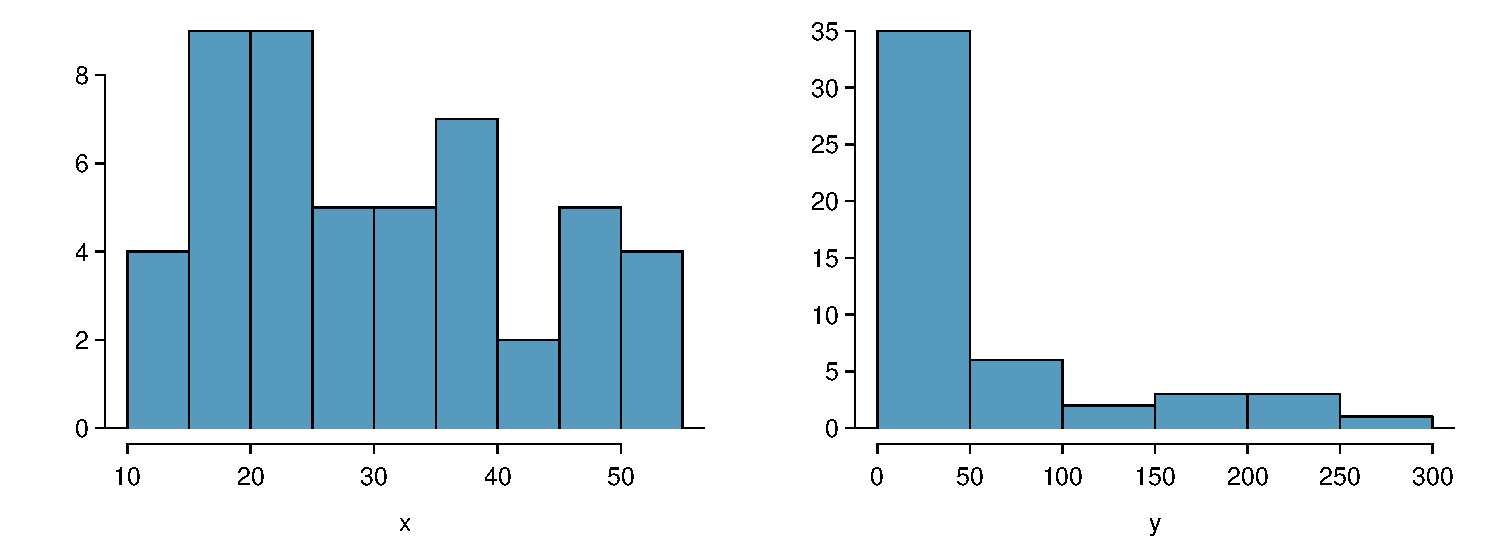
\includegraphics[width=\textwidth]{RegressionExtras/figures/nonlinear/nonlinear1-2}
\caption{Histograms for both the $x$ and $y$ variables from the left panel of Figure~\ref{nonlinear}.}
\label{nonlinear1-2}
\end{figure}

\begin{figure}
\centering
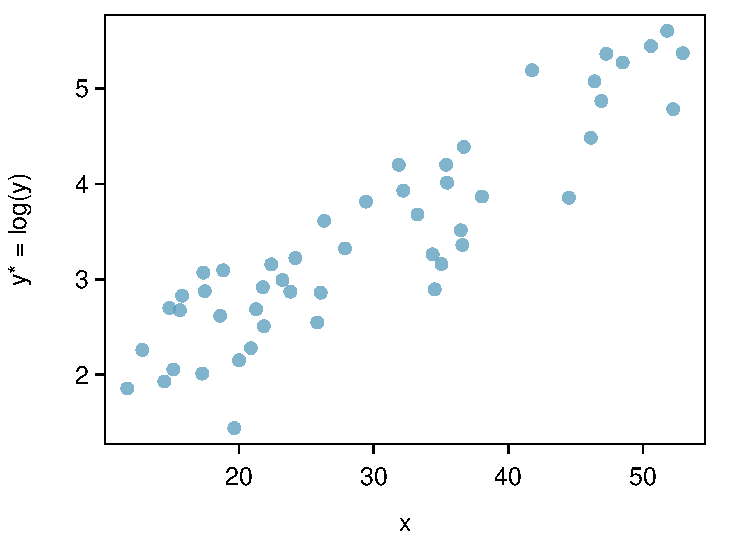
\includegraphics[width=0.7\textwidth]{RegressionExtras/figures/nonlinear/nonlinear1-3}
\caption{A plot of $y^\star$ (the result of transforming $y$ by taking the natural logarithm $\log y$) against $x$. The relationship between $y^\star$ and $x$ appears to be linear.}
\label{nonlinear1-3}
\end{figure}

We may now readily fit a linear model to the transformed scatterplot:
\begin{align*}
\hat{y}^\star &= 1.03 + 0.08x \\
y^\star &= 1.03 + 0.08x + residuals
\end{align*}
In the first equation above, the formula has been written in the form used by \href{http://www.openintro.org/stat/textbook.php}{OpenIntro Statistics}. The second line is a more general way to write this formula. This general form is important when we are transforming data since we often want to \term{back-transform} the data. Here, we back-transform by substituting $\log(y)$ for $y^\star$ and then solve for $y$:
\begin{align*}
y^\star &= 1.03 + 0.08x + residuals \\
\log(y) &= 1.03 + 0.08x + residuals \\
y &= e^{1.03 + 0.08x + residuals}
\end{align*}
In this way, we can now enter a value for $x$ and get an estimate for what value we think $y$ will take. This fitted line is shown in Figure~\ref{nonlinear1-4}.

\begin{figure}
\centering
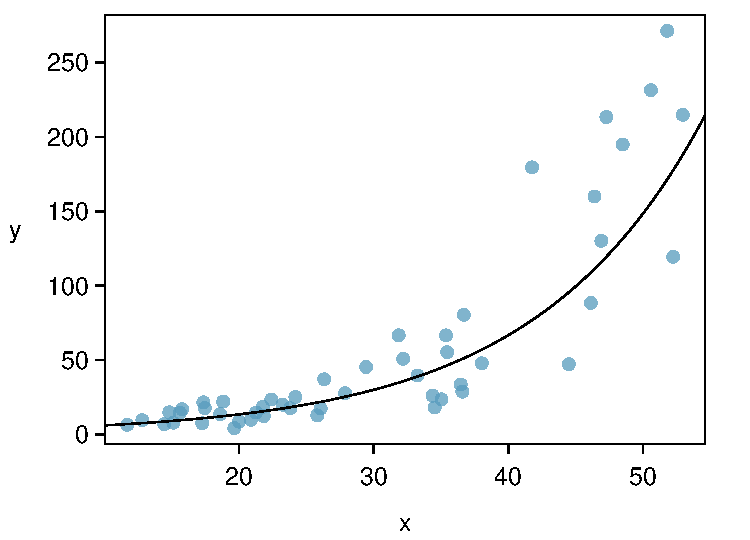
\includegraphics[width=0.7\textwidth]{RegressionExtras/figures/nonlinear/nonlinear1-4}
\caption{A nonlinear curve through the data generated by fitting a model of the form $\log y = \beta_0 + \beta_1x + residuals$, then solving for $y$.}
\label{nonlinear1-4}
\end{figure}

The predicted value for $y$ in this model should \emph{not} be confused with the expected (or mean) value of $y$ for a given value of $x$, though the result may be somewhat close. The footnote provides an explanation of the difference for the interested reader.\footnote{Suppose we collected many observations where $x=35$. This model suggests that the distribution of the corresponding $y$ values would be skewed as a result of the relationship between the residuals and the outcome $y$ being nonlinear. The model (roughly speaking) estimates the median for each value of $x$. Because the median is not the same as a mean in a skewed distribution, the model will not provide the expected value of $y$, though often times it will be close.}
%\begin{align*}
%\bar{y} &= e^{1.03 + 0.08x}\quad\text{(wrong!)} \\
%\end{align*}

\begin{tipBox}{\tipBoxTitle{Interpreting coefficients from a model that used $\log y$}
If the outcome in a model was transformed using the natural logarithm and the model fits well, then $y$ tends to grow (or decay) \term{exponentially} relative to $x$.} % For~example, in the model shown in Figure~\ref{nonlinear1-4}, a ``typical'' value for $y$ would be twice as large when $x$ is $\frac{\log2}{0.08} = 8.66$ units larger. If we compared the typical values for $y$ when $x=20$, $x=28.66$, and $x=37.32$, then $y_{x=28.66}$ would be twice as large as $y_{x=20}$, and $y_{x=37.32}$ would be \emph{four} times as large as $y_{x=20}$.}
\end{tipBox}

\begin{caution}{Transformations can be abused}
{There is a very large number of possible transformations. If we keep trying transformations until one ``works'', we have not effectively modeled our data. Rather, we have performed a complicated form of data fishing where we mine the data until we see structure. This apparent structure may just be due to chance. Therefore, think carefully about transformations before applying them.}
\end{caution}

You are once again armed with knowledge that is both powerful and dangerous. This very brief introduction to transformations should be useful for informal projects. For a more complete review of this topic, visit Chapter~8 of \emph{Practical Regression and ANOVA~in~R}, which can be found in the Free Books section on the \href{http://www.openintro.org/stat/supplements.php?feature=regression_online_extra_more_free_books}{Supplements page of openintro.org}.


\subsection{Fitting a polynomial curve}
\label{fittingAPolynomialCurve}

%A second strategy for addressing nonlinearity is to create new variables using existing variables fit a new set of variables, ones that themselves try to match the nonlinearity of the outcome $y$. It is common to try to add additional polynomial terms to the model. In effect, we generate a new set of variables $x_2=x^2$, $x_3=x^3$, and so one that we can consider adding to the model (note: we rarely use $x_3=x^3$ and beyond, though we will encounter such an example in this section).

Let's take a look at the second nonlinear relationship we saw in Figure~\ref{nonlinear}, which appears again in Figure~\ref{nonlinear2-2} with a poorly-fit straight line. Here we see what appears to be a nonlinear relationship but where the residuals would be approximately \term{homoskedastic} (constant variance) if we could reasonably model the curve of the line. This is a good signal that we want to fit a curve but not perform a transformation. We can do so by generating a \term{polynomial basis} of $x$: $x_1=x$, $x_2 = x^2$, $x_3 = x^3$, and so on. In short, we will use the variables $x_1$, $x_2$, $x_3$, ... in a multiple regression model instead of simply the original variable $x$. We should note that it is uncommon to use terms beyond $x_2 = x^2$ and very rarely beyond $x_3=x^3$.

We start by fitting a linear model to the data, where the best-fitting straight line is shown in Figure~\ref{nonlinear2-2} and summarized as
\begin{align*}
y = 0.8441 - 0.0964x + residuals
\end{align*}
Even without checking the residual plot, it is evident that this line does not fit the data well, though Table~\ref{nonlinear2-linearfitsummary} shows that the linear term is statistically significant.

\begin{figure}
\centering
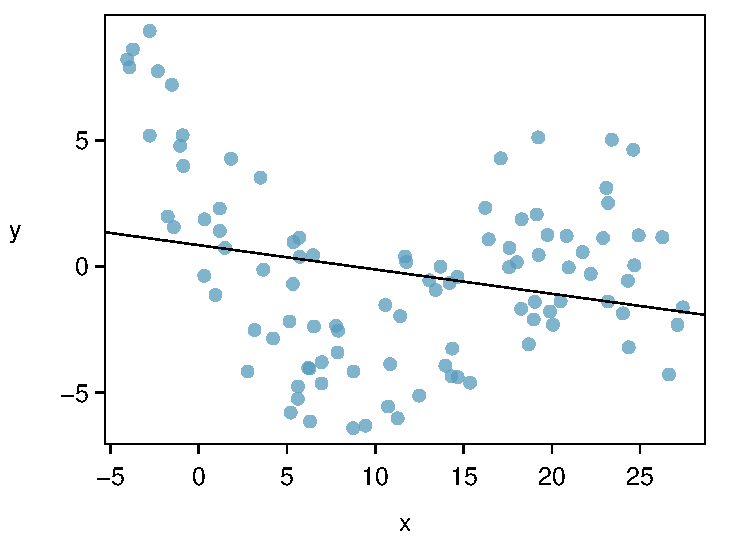
\includegraphics[width=0.6\textwidth]{RegressionExtras/figures/nonlinear/nonlinear2-2}
\caption{Scatterplot with the best-fitting straight line, which does not fit the data well.}
\label{nonlinear2-2}
\end{figure}

\begin{exercise}
Suppose you were providing feedback to someone on a project, and the colleague had fit the line to the data shown in Figure~\ref{nonlinear2-2}. Suppose also that your colleague believes this model is sufficient because the estimate for the slope is statistically significant. Explain why the model is inappropriate. One possible explanation is provided in the footnote.\footnote{Regression models require certain conditions to be met. In particular, the residuals must be independent of each other. However, when we look at the residuals from the fit in Figure~\ref{nonlinear2-2}, there is a clear trend in the residuals not captured by the straight line, meaning the independence condition is violated and the model is inadequate.}
\end{exercise}

\begin{table}
\centering
\begin{tabular}{rrrrr}
  \hline
 & Estimate & Std. Error & t value & Pr($>$$|$t$|$) \\ 
  \hline
(Intercept) & 0.8441 & 0.5799 & 1.46 & 0.1487 \\ 
  x1  & -0.0964 & 0.0397 & -2.43 & 0.0169 \\ 
   \hline
\end{tabular}
\caption{Summary for a straight line fit to the data shown in Figure~\ref{nonlinear2-2}.}
\label{nonlinear2-linearfitsummary}
\end{table}

As a next step, we'll add another variable to the model: $x_2=x^2$. This new variable is itself a transformation on the variable $x$. However, rather than substituting $x_2$ for $x$, we'll fit a multiple regression model \emph{including both variables} from the polynomial basis:
\begin{align*}
y = \beta_0 + \beta_1x_1 + \beta_2x_2 + residuals
\end{align*}
The best-fitting model of this form is shown in Figure~\ref{nonlinear2-3}, and the summary for the model is shown in Table~\ref{nonlinear2-quadfitsummary}.

\begin{figure}
\centering
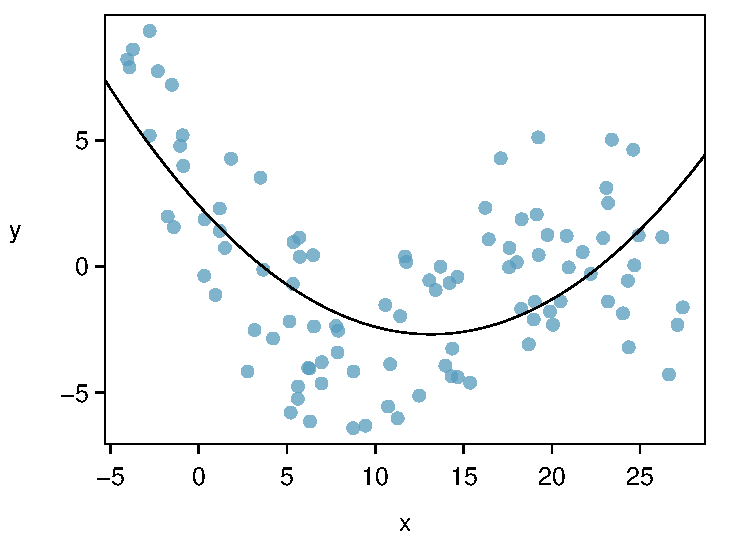
\includegraphics[width=0.65\textwidth]{RegressionExtras/figures/nonlinear/nonlinear2-3}
\caption{Scatterplot with the best-fitting quadratic line, which fits better than a straight-line but still misses some data structures. For example, the model underestimates much of the data for the range -5 to 0 and it overestimates nearly all of the data between 5 and 10.}
\label{nonlinear2-3}
\end{figure}

\begin{table}
\centering
\begin{tabular}{rrrrr}
  \hline
 & Estimate & Std. Error & t value & Pr($>$$|$t$|$) \\ 
  \hline
(Intercept) & 2.4252 & 0.5079 & 4.78 & 0.0000 \\ 
  x1  & -0.7769 & 0.0956 & -8.13 & 0.0000 \\ 
  x2  & 0.0295 & 0.0039 & 7.55 & 0.0000 \\ 
   \hline
\end{tabular}
\caption{Summary for a quadratic fit to the data shown in Figure~\ref{nonlinear2-3}.}
\label{nonlinear2-quadfitsummary}
\end{table}

\begin{example}{Write out the best fitting quadratic model using Table~\ref{nonlinear2-quadfitsummary}.}
The model may be written as
\begin{align*}
y &= 2.4252 - 0.7769x_1 + 0.0295x_2 + residuals \\
	&= 2.4252 - 0.7769x + 0.0295x^2 + residuals
\end{align*}
\end{example}

In this example a quadratic model is still insufficient, so we will try a cubic polynomial (also known as a third-order polynomial). We will try fitting a model based on a cubic polynomial:
\begin{align*}
y &= \beta_0 + \beta_1x_1 + \beta_2x_2 + \beta_3x_3 + residuals \\
	&= \beta_0 + \beta_1x + \beta_2x^2 + \beta_3x^3 + residuals
\end{align*}
Such a model is summarized in Figure~\ref{nonlinear2-4} and Table~\ref{nonlinear2-cubicfitsummary}.
\begin{figure}
\centering
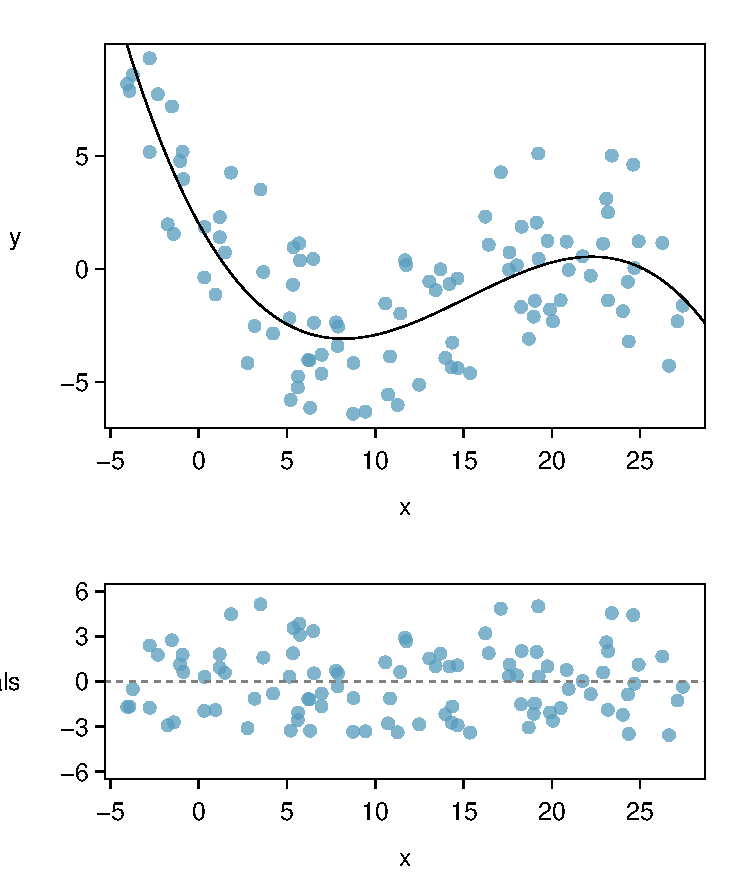
\includegraphics[width=0.65\textwidth]{RegressionExtras/figures/nonlinear/nonlinear2-4}
\caption{Scatterplot with the best-fitting cubic line. The residual plot shows no apparent structure, which is a good sign the model is fitting well.}
\label{nonlinear2-4}
\end{figure}
\begin{table}
\centering
\begin{tabular}{rrrrr}
  \hline
 & Estimate & Std. Error & t value & Pr($>$$|$t$|$) \\ 
  \hline
(Intercept) & 2.0187 & 0.4242 & 4.76 & 0.0000 \\ 
  x1 & -1.4202 & 0.1236 & -11.49 & 0.0000 \\ 
  x2 & 0.1187 & 0.0136 & 8.75 & 0.0000 \\ 
  x3 & -0.0026 & 0.0004 & -6.77 & 0.0000 \\ 
   \hline
\end{tabular}
\caption{Summary for a cubic line fit to the data shown in Figure~\ref{nonlinear2-4}}
\label{nonlinear2-cubicfitsummary}
\end{table}

\begin{exercise}
Write out the best fitting quadratic model using Table~\ref{nonlinear2-cubicfitsummary}. The solution is in the footnote.\footnote{$y = 2.0187 - 1.4202x_1 + 0.1187x_2 - 0.0026x_3 + residuals = 2.0187 - 1.4202x + 0.1187x^2 - 0.0026x^3 + residuals$}
\end{exercise}

The initial prognosis from the residual plot is that the cubic model fits very well. However, a complete analysis would include checking the model diagnostics carefully, which is a topic discussed in Section~8.3 of \href{http://www.openintro.org/stat/textbook.php}{OpenIntro Statistics}.

\begin{tipBox}{\tipBoxTitle{Stick with lower-order polynomials}
If you want to try out using a polynomial term in your model, consider $x^2$ and perhaps $x^3$ if the model is still not a good fit. If a cubic polynomial will not model your data well, then be very cautious about trying higher-order polynomials. Instead, consider learning about regression splines, kernel smoothing, or some other statistical technique. See the textbook \href{http://www.openintro.org/stat/supplements.php?feature=regression_online_extra_more_free_books}{Elements of Statistical Learning} for more information on advanced modeling techniques.}
\end{tipBox} 

\begin{caution}{Do not extrapolate with transformed models or models that use polynomial terms}
{Extrapolation is already treacherous for any model, but it can be much worse for transformed data or data that includes polynomial terms, as the model can deviate very rapidly from the typical values observed in the original data set.}
\end{caution}

































